\chapter{Interactive v1 Workload}
\label{sec:interactive-v1}

This workload consists of a set of relatively complex read-only queries, that touch a significant
amount of data -- often the two-step friendship neighbourhood and associated messages --, but typically in close proximity to a single node. Hence, the query complexity is sublinear to the dataset size.

The LDBC SNB Interactive workload consists of three query classes:

\begin{itemize}
\item \textbf{Complex read-only queries.} See \autoref{sec:interactive-v1-complex-reads}.
\item \textbf{Short read-only queries.} See \autoref{sec:interactive-v1-short-reads}.
\item \textbf{Insert operations.} See \autoref{sec:insert-operations}.
\end{itemize}

\subsection*{Related Publications}

A detailed description of the workload (covering reads and inserts) is available in the paper published at \mbox{SIGMOD} 2015~\cite{DBLP:conf/sigmod/ErlingALCGPPB15}. The ACID Test Suite was first published at TPCTC 2020~\cite{DBLP:conf/tpctc/WaudbySKMBS20}.
\iftoggle{StandaloneWorkloadSpecification}{}{
    It is part of this specification in \autoref{sec:acid-test-suite}.
}

%%%%%%%%%%%%%%%%%%%%%%%%%%%%%%%%%%%%%%%%%%%%%%%%%%%%%%%%%%%%%%%%%%%%%%%%%%%%%%
%%%%%%%%%%%%%%%%%%%%%%%%%%%%%%%%%%%%%%%%%%%%%%%%%%%%%%%%%%%%%%%%%%%%%%%%%%%%%%
%%%%%%%%%%%%%%%%%%%%%%%%%%%%%%%%%%%%%%%%%%%%%%%%%%%%%%%%%%%%%%%%%%%%%%%%%%%%%%

\section{Complex Reads}
\label{sec:interactive-complex-reads}

\input{interactive-v1-complex-reads}

%%%%%%%%%%%%%%%%%%%%%%%%%%%%%%%%%%%%%%%%%%%%%%%%%%%%%%%%%%%%%%%%%%%%%%%%%%%%%%
%%%%%%%%%%%%%%%%%%%%%%%%%%%%%%%%%%%%%%%%%%%%%%%%%%%%%%%%%%%%%%%%%%%%%%%%%%%%%%
%%%%%%%%%%%%%%%%%%%%%%%%%%%%%%%%%%%%%%%%%%%%%%%%%%%%%%%%%%%%%%%%%%%%%%%%%%%%%%

\section{Short Reads}
\label{sec:interactive-v1-short-reads}

\renewcommand*{\arraystretch}{1.1}

\label{sec:interactive-short-read-01}
\noindent\begin{tabularx}{\queryCardWidth}{|>{\queryPropertyCell}c|X|}
	\hline
	query & Interactive / short / 1 \\ \hline
%
	title & Person Profile \\ \hline
%
    pattern & \hfill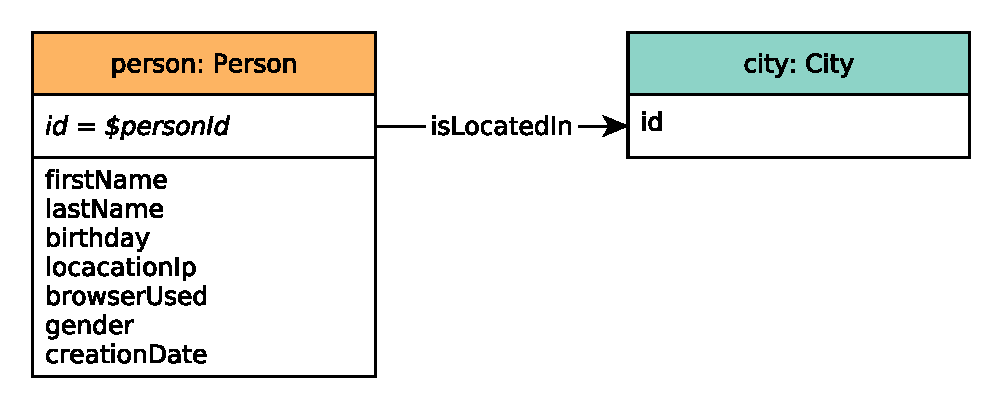
\includegraphics[scale=\patternscale,margin=0cm .2cm]{patterns/interactive-short-read-01}\hfill\vadjust{} \\ \hline
%
	desc. & Given a start Person, retrieve their first name, last name, birthday, IP
address, browser, and city of residence.
 \\ \hline
%
	
%
    
        params &
        \innerCardVSpace{\begin{tabularx}{\attributeCardWidth}{|>{\paramNumberCell}c|>{\varNameCell}M|>{\typeCell}m{\typeWidth}|Y|} \hline
        \cellcolor{parameter} \color{white} \footnotesize $\mathsf{1}$ &Person.id& ID &  \\ \hline
        \end{tabularx}}\innerCardVSpace \\ \hline
	
%
	
        result &
        \innerCardVSpace{\begin{tabularx}{\attributeCardWidth}{|>{\resultNumberCell}c|>{\varNameCell}M|>{\typeCell}m{\typeWidth}|>{\resultOriginCell}c|Y|} \hline
        $\mathsf{1}$ & Person.firstName & String &R&
                 \\ \hline
        $\mathsf{2}$ & Person.lastName & String &R&
                 \\ \hline
        $\mathsf{3}$ & Person.birthDay & Date &R&
                 \\ \hline
        $\mathsf{4}$ & Person.locationIP & String &R&
                 \\ \hline
        $\mathsf{5}$ & Person.browserUsed & String &R&
                 \\ \hline
        $\mathsf{6}$ & Person-isLocatedIn->Place.id & 32-bit Integer &R&
                 \\ \hline
        $\mathsf{7}$ & Person.gender & String &R&
                 \\ \hline
        $\mathsf{8}$ & Person.creationDate & DateTime &R&
                 \\ \hline
        \end{tabularx}}\innerCardVSpace \\ \hline
	
%
	%
	%
	%
    %
\end{tabularx}
\queryCardVSpace
\renewcommand*{\arraystretch}{1.1}

\noindent\begin{tabularx}{17cm}{|p{1.95cm}|X|}
	\hline
	workload    & Interactive / short \\ \hline
%
	query       & 2 \\ \hline
%
	title       & Person Recent Messages \\ \hline
%
    pattern     & \hfill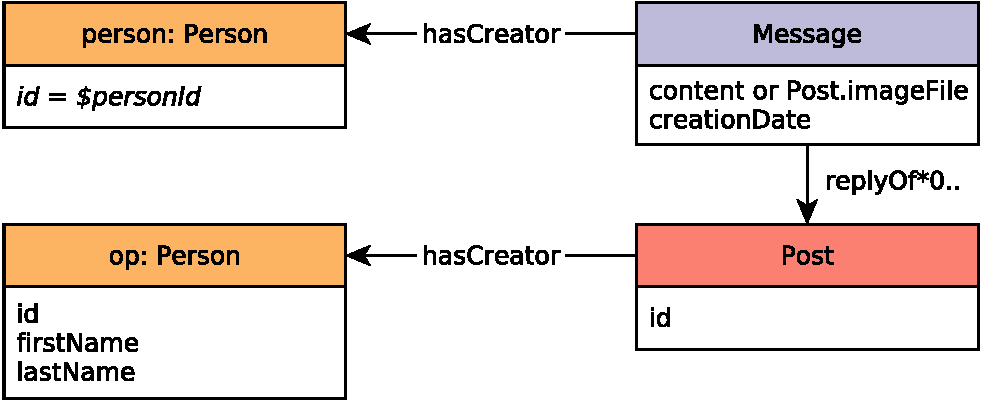
\includegraphics[scale=\patternscale,margin=0cm .2cm]{patterns/interactive-short-read-02}\hfill\vadjust{} \\ \hline
%
	description & Given a start Person, retrieve the last 10 Messages created by that
user. For each message, return that message, the original post in its
conversation, and the author of that post. If any of the Messages is a
Post, then the original Post will be the same Message, i.e.~that Message
will appear twice in that result.
 \\ \hline
%
	
%
	parameters  &
	\vspace{1.1ex}{\begin{tabularx}{14.2cm}{|c|M|m{2cm}|Y|} \hline
	\cellcolor{black!70} \color{white} $\mathsf{1}$ & \varname{Person.id} & \cellcolor{gray!20} \vartype{ID} &  \\ \hline
	\end{tabularx}}\vspace{1.1ex} \\ \hline
%
	
	result      &
	\vspace{1.1ex}{\begin{tabularx}{14.2cm}{|c|M|m{2cm}|Y|} \hline
	\cellcolor{black!70} \color{white} $\mathsf{1}$ & \varname{Message.id} & \cellcolor{gray!20} \vartype{64-bit Integer} &  \\ \hline
	\cellcolor{black!70} \color{white} $\mathsf{2}$ & \varname{Message.content or Post.imageFile} & \cellcolor{gray!20} \vartype{String} &  \\ \hline
	\cellcolor{black!70} \color{white} $\mathsf{3}$ & \varname{Message.creationDate} & \cellcolor{gray!20} \vartype{DateTime} &  \\ \hline
	\cellcolor{black!70} \color{white} $\mathsf{4}$ & \varname{Post.id or Comment-replyOf*->Post.id} & \cellcolor{gray!20} \vartype{ID} &  \\ \hline
	\cellcolor{black!70} \color{white} $\mathsf{5}$ & \varname{Post-hasCreator->Person.id or Comment-replyOf*->Post-hasCreator->Person.id} & \cellcolor{gray!20} \vartype{ID} &  \\ \hline
	\cellcolor{black!70} \color{white} $\mathsf{6}$ & \varname{Post-hasCreator->Person.firstName or Comment-replyOf*->Post-hasCreator->Person.firstName} & \cellcolor{gray!20} \vartype{String} &  \\ \hline
	\cellcolor{black!70} \color{white} $\mathsf{7}$ & \varname{Post-hasCreator->Person.lastName or Comment-replyOf*->Post-hasCreator->Person.lastName} & \cellcolor{gray!20} \vartype{String} &  \\ \hline
	\end{tabularx}}\vspace{1.1ex} \\ \hline
	
%
	sort        &
	\vspace{1.1ex}{\begin{tabular}{|c|l|c|} \hline
	\cellcolor{black!70} \color{white} $\mathsf{1}$ & \varname{Message.creationDate} & \cellcolor{gray!20} $\desc$ \\ \hline
	\cellcolor{black!70} \color{white} $\mathsf{2}$ & \varname{Message.id} & \cellcolor{gray!20} $\desc$ \\ \hline
	\end{tabular}}\vspace{1.1ex} \\ \hline
	%
	%
	%
\end{tabularx}
\vspace{2ex}
\renewcommand*{\arraystretch}{1.1}

\subsection*{Interactive / short / 3}
\label{section:interactive-short-read-03}

% change \emph{} to use sans-serif font
\let\oldemph\emph
\renewcommand{\emph}[1]{{\footnotesize \sf #1}}



\noindent\begin{tabularx}{\queryCardWidth}{|>{\queryPropertyCell}p{\queryPropertyCellWidth}|X|}
	\hline
	query & Interactive / short / 3 \\ \hline
%
	title & Person Friends \\ \hline
%
	pattern & \multicolumn{1}{c|}{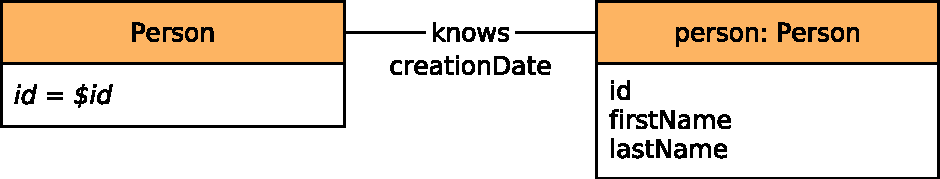
\includegraphics[scale=\patternscale,margin=0cm .2cm]{patterns/interactive-short-read-03}} \\ \hline
%
	desc. & Given a start Person, retrieve all of their friends, and the date at
which they became friends.
 \\ \hline
%
	
		params &
		\innerCardVSpace{\begin{tabularx}{\attributeCardWidth}{|>{\paramNumberCell}c|>{\varNameCell}M|>{\typeCell}m{\typeWidth}|Y|} \hline
		$\mathsf{1}$ & Person.id
 & ID
 &  \\ \hline
		\end{tabularx}}\innerCardVSpace \\ \hline
	
%
	
		result &
		\innerCardVSpace{\begin{tabularx}{\attributeCardWidth}{|>{\resultNumberCell}c|>{\varNameCell}M|>{\typeCell}m{\typeWidth}|>{\resultOriginCell}c|Y|} \hline
		$\mathsf{1}$ & Person.id & ID & R &
				 \\ \hline
		$\mathsf{2}$ & Person.firstName & String & R &
				 \\ \hline
		$\mathsf{3}$ & Person.lastName & String & R &
				 \\ \hline
		$\mathsf{4}$ & Knows.creationDate & DateTime & R &
				 \\ \hline
		\end{tabularx}}\innerCardVSpace \\ \hline
	
%
	
		sort		&
		\innerCardVSpace{\begin{tabularx}{\attributeCardWidth}{|>{\sortNumberCell}c|>{\varNameCell}M|>{\directionCell}c|Y|} \hline
		$\mathsf{1}$ & Knows.creationDate
 & $\desc
$ &  \\ \hline
		$\mathsf{2}$ & Person.id
 & $\asc
$ &  \\ \hline
		\end{tabularx}}\innerCardVSpace \\ \hline
	%
	%
	%
	%
\end{tabularx}
\queryCardVSpace

% change \emph back to the old one
\renewcommand{\emph}[1]{\oldemph{#1}}
\renewcommand*{\arraystretch}{1.1}

\subsection*{Interactive / short / 4}
\label{section:interactive-short-read-04}

% change \emph{} to use sans-serif font
\let\oldemph\emph
\renewcommand{\emph}[1]{{\footnotesize \sf #1}}



\noindent\begin{tabularx}{\queryCardWidth}{|>{\queryPropertyCell}p{\queryPropertyCellWidth}|X|}
	\hline
	query & Interactive / short / 4 \\ \hline
%
	title & Message Content \\ \hline
%
	pattern & \hfill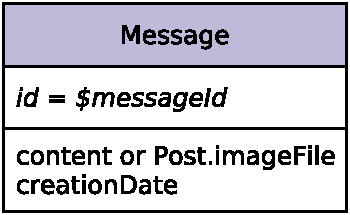
\includegraphics[scale=\patternscale,margin=0cm .2cm]{patterns/interactive-short-read-04}\hfill\vadjust{} \\ \hline
%
	desc. & Given a Message, retrieve its content and creation date.
 \\ \hline
%
	
		params &
		\innerCardVSpace{\begin{tabularx}{\attributeCardWidth}{|>{\paramNumberCell}c|>{\varNameCell}M|>{\typeCell}m{\typeWidth}|Y|} \hline
		$\mathsf{1}$ & Message.id
 & ID
 &  \\ \hline
		\end{tabularx}}\innerCardVSpace \\ \hline
	
%
	
		result &
		\innerCardVSpace{\begin{tabularx}{\attributeCardWidth}{|>{\resultNumberCell}c|>{\varNameCell}M|>{\typeCell}m{\typeWidth}|>{\resultOriginCell}c|Y|} \hline
		$\mathsf{1}$ & Message.creationDate & ID & R &
				 \\ \hline
		$\mathsf{2}$ & Message.content or Post.imageFile & String & R &
				 \\ \hline
		\end{tabularx}}\innerCardVSpace \\ \hline
	
%
	%
	%
	%
	%
\end{tabularx}
\queryCardVSpace

% change \emph back to the old one
\renewcommand{\emph}[1]{\oldemph{#1}}
\renewcommand*{\arraystretch}{1.1}

\noindent\begin{tabularx}{17cm}{|>{\small \sf}c|X|}
	\hline
	query    & Interactive / short / 5 \\ \hline
%
	title       & Message Creator \\ \hline
%
    pattern     & \hfill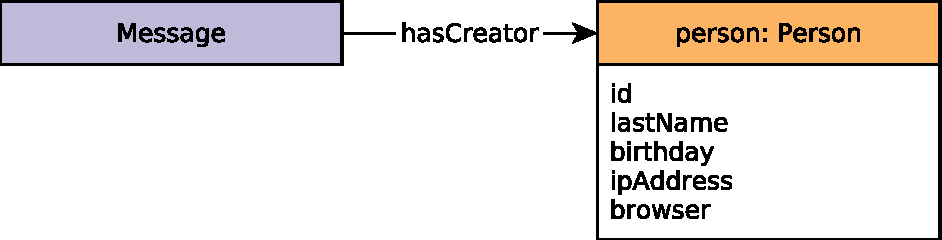
\includegraphics[scale=\patternscale,margin=0cm .2cm]{patterns/interactive-short-read-05}\hfill\vadjust{} \\ \hline
%
	desc. & Given a Message, retrieve its author.
 \\ \hline
%
	
%
	params.  &
	\vspace{1.1ex}{\begin{tabularx}{14.66cm}{|c|M|m{2cm}|Y|} \hline
	\cellcolor{parameter} \color{white} $\mathsf{1}$ & \varname{Message.id} & \cellcolor{gray!20} \vartype{ID} &  \\ \hline
	\end{tabularx}}\vspace{1.1ex} \\ \hline
%
	
	result      &
	\vspace{1.1ex}{\begin{tabularx}{14.66cm}{|c|M|m{2cm}|c|Y|} \hline
	\cellcolor{result} \color{white} $\mathsf{1}$ & \varname{Message-hasCreator->Person.id} & \cellcolor{gray!20} \vartype{ID} &
	    \texttt{R} &
	     \\ \hline
	\cellcolor{result} \color{white} $\mathsf{2}$ & \varname{Message-hasCreator->Person.firstName} & \cellcolor{gray!20} \vartype{String} &
	    \texttt{R} &
	     \\ \hline
	\cellcolor{result} \color{white} $\mathsf{3}$ & \varname{Message-hasCreator->Person.lastName} & \cellcolor{gray!20} \vartype{String} &
	    \texttt{R} &
	     \\ \hline
	\end{tabularx}}\vspace{1.1ex} \\ \hline
	
%
	%
	%
	%
    %
\end{tabularx}
\vspace{2ex}
\renewcommand*{\arraystretch}{1.1}

\subsection*{Interactive / short / 6}
\label{sec:interactive-short-read-06}

\noindent\begin{tabularx}{\queryCardWidth}{|>{\queryPropertyCell}c|X|}
	\hline
	query & Interactive / short / 6 \\ \hline
%
	title & Message Forum \\ \hline
%
    pattern & \hfill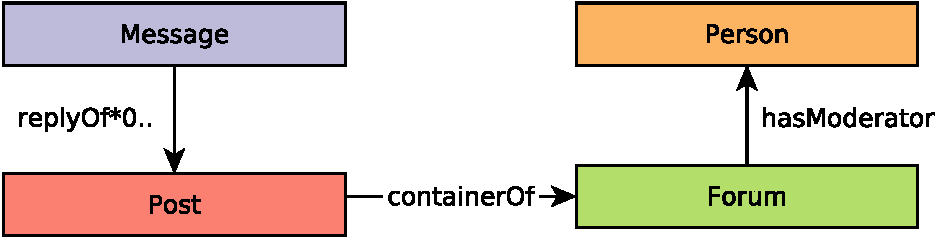
\includegraphics[scale=\patternscale,margin=0cm .2cm]{patterns/interactive-short-read-06}\hfill\vadjust{} \\ \hline
%
	desc. & Given a Message, retrieve the Forum that contains it and the Person that
moderates that forum. Since comments are not directly contained in
forums, for comments, return the forum containing the original post in
the thread which the comment is replying to.
 \\ \hline
%
	
%
    
        params &
        \innerCardVSpace{\begin{tabularx}{\attributeCardWidth}{|>{\paramNumberCell}c|>{\varNameCell}M|>{\typeCell}m{\typeWidth}|Y|} \hline
        \cellcolor{parameter} \color{white} \footnotesize $\mathsf{1}$ &Message.id& ID &  \\ \hline
        \end{tabularx}}\innerCardVSpace \\ \hline
	
%
	
        result &
        \innerCardVSpace{\begin{tabularx}{\attributeCardWidth}{|>{\resultNumberCell}c|>{\varNameCell}M|>{\typeCell}m{\typeWidth}|>{\resultOriginCell}c|Y|} \hline
        $\mathsf{1}$ & Message<-containerOf-Forum.id & ID &R&
                 \\ \hline
        $\mathsf{2}$ & Message<-containerOf-Forum.title & String &R&
                 \\ \hline
        $\mathsf{3}$ & Message<-containerOf-Forum-hasModerator->Person.id & ID &R&
                 \\ \hline
        $\mathsf{4}$ & Message<-containerOf-Forum-hasModerator->Person.firstName & String &R&
                 \\ \hline
        $\mathsf{5}$ & Message<-containerOf-Forum-hasModerator->Person.lastName & String &R&
                 \\ \hline
        \end{tabularx}}\innerCardVSpace \\ \hline
	
%
	%
	%
	%
    %
\end{tabularx}
\queryCardVSpace
\renewcommand*{\arraystretch}{1.1}

\subsection*{Interactive / short / 7}
\label{section:interactive-short-read-07}

% change \emph{} to use sans-serif font
\let\oldemph\emph
\renewcommand{\emph}[1]{{\footnotesize \sf #1}}



\noindent\begin{tabularx}{\queryCardWidth}{|>{\queryPropertyCell}p{\queryPropertyCellWidth}|X|}
	\hline
	query & Interactive / short / 7 \\ \hline
%
	title & Message Replies
 \\ \hline
%
	pattern & \hfill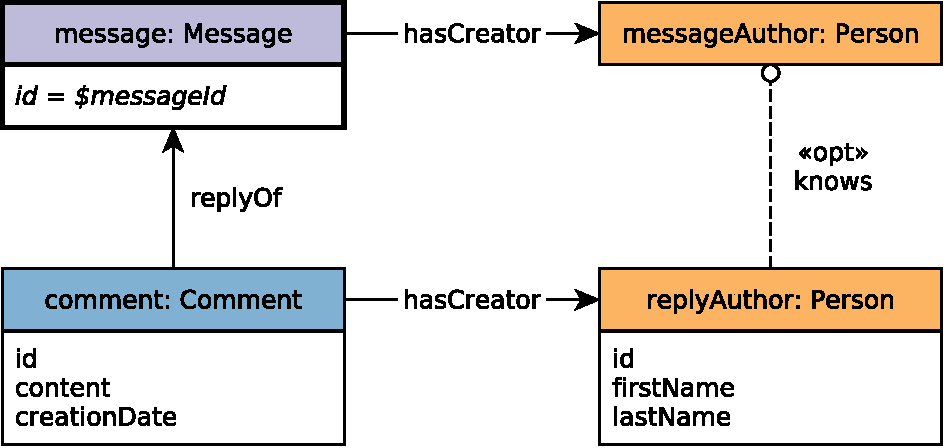
\includegraphics[scale=\patternscale,margin=0cm .2cm]{patterns/interactive-short-read-07}\hfill\vadjust{} \\ \hline
%
	desc. & Given a Message, retrieve the (1-hop) Comments that reply to it.

In addition, return a boolean flag \texttt{knows} indicating if the
author of the reply knows the author of the original message. If author
is same as original author, return false for \texttt{knows} flag.
 \\ \hline
%
	
		params &
		\innerCardVSpace{\begin{tabularx}{\attributeCardWidth}{|>{\paramNumberCell}c|>{\varNameCell}M|>{\typeCell}m{\typeWidth}|Y|} \hline
		$\mathsf{1}$ & Message.id
 & ID
 &  \\ \hline
		\end{tabularx}}\innerCardVSpace \\ \hline
	
%
	
		result &
		\innerCardVSpace{\begin{tabularx}{\attributeCardWidth}{|>{\resultNumberCell}c|>{\varNameCell}M|>{\typeCell}m{\typeWidth}|>{\resultOriginCell}c|Y|} \hline
		$\mathsf{1}$ & Message\textless{}-replyOf-Comment.id & ID & R &
				 \\ \hline
		$\mathsf{2}$ & Message\textless{}-replyOf-Comment.content & String & R &
				 \\ \hline
		$\mathsf{3}$ & Message\textless{}-replyOf-Comment.creationDate & DateTime & R &
				 \\ \hline
		$\mathsf{4}$ & Comment-hasCreator-\textgreater{}Person.id & ID & R &
				 \\ \hline
		$\mathsf{5}$ & Comment-hasCreator-\textgreater{}Person.firstName & String & R &
				 \\ \hline
		$\mathsf{6}$ & Comment-hasCreator-\textgreater{}Person.lastName & String & R &
				 \\ \hline
		$\mathsf{7}$ & knows & Boolean & C &
				Original message author knows reply author
 \\ \hline
		\end{tabularx}}\innerCardVSpace \\ \hline
	
%
	
		sort		&
		\innerCardVSpace{\begin{tabularx}{\attributeCardWidth}{|>{\sortNumberCell}c|>{\varNameCell}M|>{\directionCell}c|Y|} \hline
		$\mathsf{1}$ & Message\textless{}-replyOf-Comment.creationDate
 & $\desc
$ &  \\ \hline
		$\mathsf{2}$ & Message-hasCreator-\textgreater{}Person.id
 & $\asc
$ &  \\ \hline
		\end{tabularx}}\innerCardVSpace \\ \hline
	%
	%
	%
	%
\end{tabularx}
\queryCardVSpace

% change \emph back to the old one
\renewcommand{\emph}[1]{\oldemph{#1}}


%%%%%%%%%%%%%%%%%%%%%%%%%%%%%%%%%%%%%%%%%%%%%%%%%%%%%%%%%%%%%%%%%%%%%%%%%%%%%%
%%%%%%%%%%%%%%%%%%%%%%%%%%%%%%%%%%%%%%%%%%%%%%%%%%%%%%%%%%%%%%%%%%%%%%%%%%%%%%
%%%%%%%%%%%%%%%%%%%%%%%%%%%%%%%%%%%%%%%%%%%%%%%%%%%%%%%%%%%%%%%%%%%%%%%%%%%%%%

\iftoggle{StandaloneWorkloadSpecification}{
    \section{Insert Operations}
    \label{sec:insert-operations}
    \input{query-cards/insert-01}
\input{query-cards/insert-02}
\input{query-cards/insert-03}
\input{query-cards/insert-04}
\input{query-cards/insert-05}
\input{query-cards/insert-06}
\input{query-cards/insert-07}
\input{query-cards/insert-08}

}

%%%%%%%%%%%%%%%%%%%%%%%%%%%%%%%%%%%%%%%%%%%%%%%%%%%%%%%%%%%%%%%%%%%%%%%%%%%%%%
%%%%%%%%%%%%%%%%%%%%%%%%%%%%%%%%%%%%%%%%%%%%%%%%%%%%%%%%%%%%%%%%%%%%%%%%%%%%%%
%%%%%%%%%%%%%%%%%%%%%%%%%%%%%%%%%%%%%%%%%%%%%%%%%%%%%%%%%%%%%%%%%%%%%%%%%%%%%%

\section{Workload Definition}
\label{sec:interactive-workload-definition}

The \emph{Test Driver} is in charge of the execution of the Interactive Workload.
At the beginning of the execution, the Test Driver creates a query mix by
assigning to each query instance, a query issue time and a set of parameters
taken from the generated substitution parameter set described above.  

Query issue times have to be carefully assigned.  Although substitution
parameters are chosen in such a way that queries of the same type take similar
time, not all query types have the same complexity and touch the same amount of
data, which causes them to scale differently for the different scale factors.
Therefore, if all query instances, regardless of their type, are issued
at the same rate, those more complex queries will dominate the execution's
result, making faster query types purposeless. To avoid this situation, each
query type is executed at a different rate. The way the execution rate is decided,
also depends on the nature of the query: complex read, short read or update.

Update queries' issue times are taken from the update streams generated by the
data generator. These are the times where the actual event happened during the
simulation of the social network. Complex reads' times are expressed in terms
of update operations. For each complex read query type, a frequency value is
assigned which specifies the relation between the number of updates performed
per complex read. \autoref{table:freqs} shows the frequencies for each complex query and SF used in the Interactive workload (\autoref{sec:interactive}).

%\todo{Should we define frequencies for SF0.1 and SF0.3? No, those are for testing, not benchmarking.}

\begin{table}[htb]
    \centering
    \begin{tabular}{|r|r|r|r|r|r|r|r|r|}
        \hline
        \textbf{Query} & \textbf{SF1} & \textbf{SF3} & \textbf{SF10} & \textbf{SF30} & \textbf{SF100} & \textbf{SF300} & \textbf{SF\numprint{1000}} & \textbf{SF\numprint{3000}} \\\hline\hline
        1              & 26           & 26           & 26            & 26            & 26             & 26             & 26                         & 26                         \\\hline
        2              & 37           & 37           & 37            & 37            & 37             & 37             & 37                         & 37                         \\\hline
        3              & 69           & 79           & 92            & 106           & 123            & 142            & 165                        & 189                        \\\hline
        4              & 36           & 36           & 36            & 36            & 36             & 36             & 36                         & 36                         \\\hline
        5              & 57           & 61           & 66            & 72            & 78             & 84             & 91                         & 98                         \\\hline
        6              & 129          & 172          & 236           & 316           & 434            & 580            & 796                        & 1063                       \\\hline
        7              & 87           & 72           & 54            & 48            & 38             & 32             & 25                         & 21                         \\\hline
        8              & 45           & 27           & 15            & 9             & 5              & 3              & 1                          & 1                          \\\hline
        9              & 157          & 209          & 287           & 384           & 527            & 705            & 967                        & 1292                       \\\hline
        10             & 30           & 32           & 35            & 37            & 40             & 44             & 47                         & 51                         \\\hline
        11             & 16           & 17           & 19            & 20            & 22             & 24             & 26                         & 28                         \\\hline
        12             & 44           & 44           & 44            & 44            & 44             & 44             & 44                         & 44                         \\\hline
        13             & 19           & 19           & 19            & 19            & 19             & 19             & 19                         & 19                         \\\hline
        14             & 49           & 49           & 49            & 49            & 49             & 49             & 49                         & 49                         \\\hline
    \end{tabular}
    \caption{Frequencies for each Interactive complex query and SF.}
    \label{table:freqs}
\end{table}


Finally, short reads are inserted in order to balance the ratio between reads
and writes, and to simulate the behavior of a real user of the social network.
For each complex read instance, a sequence of short reads is planned. There are two
types of short read sequences: Person centric and Message centric. Depending on
the type of the complex read, one of them is chosen. Each sequence consists of
a set of short reads which are issued in a row. The issue time assigned to each
short read in the sequence is determined at run time, and is based on the
completion time of the complex read it depends on. 
The substitution parameters for short reads are taken from the results of previously
executed queries.

\begin{itemize}
\item Complex reads:
    \queryRefCard{interactive-complex-read-01}{IC}{1}
    \queryRefCard{interactive-complex-read-02}{IC}{2}
    \queryRefCard{interactive-complex-read-03}{IC}{3}
    \queryRefCard{interactive-complex-read-07}{IC}{7}
    \queryRefCard{interactive-complex-read-08}{IC}{8}
    \queryRefCard{interactive-complex-read-09}{IC}{9}
    \queryRefCard{interactive-complex-read-10}{IC}{10}
    \queryRefCard{interactive-complex-read-11}{IC}{11}
    \queryRefCard{interactive-complex-read-12}{IC}{12}
    \queryRefCard{interactive-complex-read-14-old}{IC}{14-o}
    \queryRefCard{interactive-complex-read-14-new}{IC}{14-n}
\item Short reads:
    \queryRefCard{interactive-short-read-02}{IS}{2}
    \queryRefCard{interactive-short-read-03}{IS}{3}
    \queryRefCard{interactive-short-read-05}{IS}{5}
    \queryRefCard{interactive-short-read-06}{IS}{6}
    \queryRefCard{interactive-short-read-07}{IS}{7}
\end{itemize}

For the precise connections between short and complex read queries, see \autoref{tab:short-read-after-long-read}.

Once a short read sequence is issued (and provided that sufficient substitution parameters 
exist), there is a probability that another short read  sequence is issued. 
This probability decreases for each new sequence issued. 
Since the same random number generator seed is used across
executions, the workload is deterministic.

\begin{table}[H]
    \centering
    \begin{tabular}{|l|c|c|c|c|c|c|c|}
        \hline
        \bf Read query & \bf S1 & \bf  S2 & \bf S3 & \bf S4 & \bf S5 & \bf S6 & \bf S7 \\ \hline
        Q1             & \yes   & \yes    & \yes   &        &        &        &        \\ \hline
        Q2             & \yes   & \yes    & \yes   & \yes   & \yes   & \yes   & \yes   \\ \hline
        Q3             & \yes   & \yes    & \yes   &        &        &        &        \\ \hline
        Q7             & \yes   & \yes    & \yes   & \yes   & \yes   & \yes   & \yes   \\ \hline
        Q8             & \yes   & \yes    & \yes   & \yes   & \yes   & \yes   & \yes   \\ \hline
        Q9             & \yes   & \yes    & \yes   & \yes   & \yes   & \yes   & \yes   \\ \hline
        Q10            & \yes   & \yes    & \yes   &        &        &        &        \\ \hline
        Q11            & \yes   & \yes    & \yes   &        &        &        &        \\ \hline
        Q12            & \yes   & \yes    & \yes   &        &        &        &        \\ \hline
        Q14            & \yes   & \yes    & \yes   &        &        &        &        \\ \hline
        IS2            & \yes   & \yes    & \yes   & \yes   & \yes   & \yes   & \yes   \\ \hline
        IS3            & \yes   & \yes    & \yes   &        &        &        &        \\ \hline
        IS5            & \yes   & \yes    & \yes   &        &        &        &        \\ \hline
        IS6            & \yes   & \yes    & \yes   &        &        &        &        \\ \hline
        IS7            & \yes   & \yes    & \yes   & \yes   & \yes   & \yes   & \yes   \\ \hline
    \end{tabular}
    \caption{Short read queries executed after read query.}
    \label{tab:short-read-after-long-read}
\end{table}


The specified frequencies, implicitly define the query ratios between queries
of different types, as well as a default target throughput. However, the Test
Sponsor may specify a different target throughput to test,  by ``squeezing''
together or ``stretching'' apart the queries of the workload. This is
achieved by means of the ``Time Compression Ratio'' that is multiplied by the
frequencies (see \autoref{table:freqs}).  Therefore, different
throughputs can be tested while maintaining the relative ratios between the
different query types.


